\section{NDN Overview\label{sec:ccn-intro}}
%Named Data Networking (NDN) is a network architecture which aims to replace IP architecture by replacing IP�s host-to-host data delivery model with pull-based information retrieval model. In IP in order to retrieve data, data consumer have to know endpoint location of the desired data, in NDN all they have to know is data name. Names are hierarchical (non-flat) application-defined string names that are used for forwarding, routing and caching. A canonical NDN name looks in a following way: /ndn/ucla/CSdept/faculty/Lixia/webpage.

In this section we briefly introduce NDN with a focus on its stateful forwarding plane (for more details refer to \cite{ndn-conext, ndn-tr, adaptive-forwarding}).
NDN is a receiver-driven, data-centric communication protocol.
All communication in NDN is performed using two distinct types of packets: \textit{Interest} and \textit{Data}. Both types of packets carry a \textit{name}, which uniquely identifies a piece of data that can be carried in one Data packet. Somewhat similar to domain names, data names in NDN are hierarchically structured and an example name of a youtube video would look like: \ndnName{/youtube/videos/www/1234.flv}.

To retrieve Data, a consumer request it by sending an Interest packet with the name of the desired content in it.
Routers use this name to route the Interest towards likely sources, and a Data packet, if any, whose name matches the name in the Interest is returned to the consumer by following the reverse path of the interest. Similar to IP, routing in NDN is based on longest prefix match, but, unlike IP,  communication path is always symmetric. An Interest is ``satisfied'' when it is matched with a Data packet.

Each NDN router maintains three major data structures:
\begin{itemize}
\item \textit{Pending Interest Table (PIT)} holds all ``not yet satisfied'' Interests that have been sent upstream towards data producers. Each entry in PIT contains a list of incoming, and outgoing, physical interfaces; the former enables multicast Data delivery, and the latter is needed when the same Interest is forwarded along multiple paths.
\item \textit{Forwarding Interest Base (FIB)} maps name prefixes to one or multiple physical network interfaces, defining allowed %(multipath)
 directions where to forward Interests. 
% Having one-to-many relationship in this table allows multipath forwarding of Interests.}
\item \textit{Content Store (CS)} temporarily buffers Data packets that pass through this node, allowing fast Data retrieval by different consumers.
\end{itemize}

When a router receives an Interest packet, it first checks whether there is a matching Data in its CS.
If a match is found, the Data is sent back to the incoming interface of the Interest packet.
If not, the Interest name is checked against the entries in the PIT. 
If the name exists in the PIT already, then it can be either a duplicate Interest (identified by a long random number each Interest carries) that should be dropped,
or an Interest from another consumer asking for the same Data which requires the incoming interface of this Interest to be added to the existing PIT entry (i.e., ``collapsing'' multiple Interests for the same content into one PIT entry).
If the name does not exist in the PIT, the Interest is added into the PIT and forwarded to the interface chosen by the strategy module, which uses FIB as input for its decision.

When a Data packet is received, its name is used to look up the PIT.
If a matching PIT entry is found,
the router sends the Data packet to the interface(s) from which the Interest was received, caches the data in the CS, and removes the PIT entry.  Otherwise, the Data packet is unsolicited and discarded. 
Each Interest also has an associated lifetime; the PIT entry is removed when the lifetime expires.
Although the maximum lifetime is specified by users, it is ultimately a router's decision how long it is willing to keep the PIT entry.  
For simplicity, we assume routers keep Interests in PIT for one second in our simulations.

%Every incoming Interest triggers a lookup in the Content Store and if the Data with matching data name have been found, it is sent back to the same physical interface from which the Interest has arrived. If CS lookup is unsuccessful, Interest must be sent further upstream and put in the PIT. However, all recurring Interests with the same prefix name are stacked together in the same PIT entry and are not sent to the upstream again until this PIT entry expires completely because of timeout. If Data returns from some upstream location it is replicated for each incoming physical interface stored in this PIT entry after that it is removed from PIT. In other words, multipath Data delivery is built-in in NDN. 


%\begin{figure}[htpb]
%  \centering
%  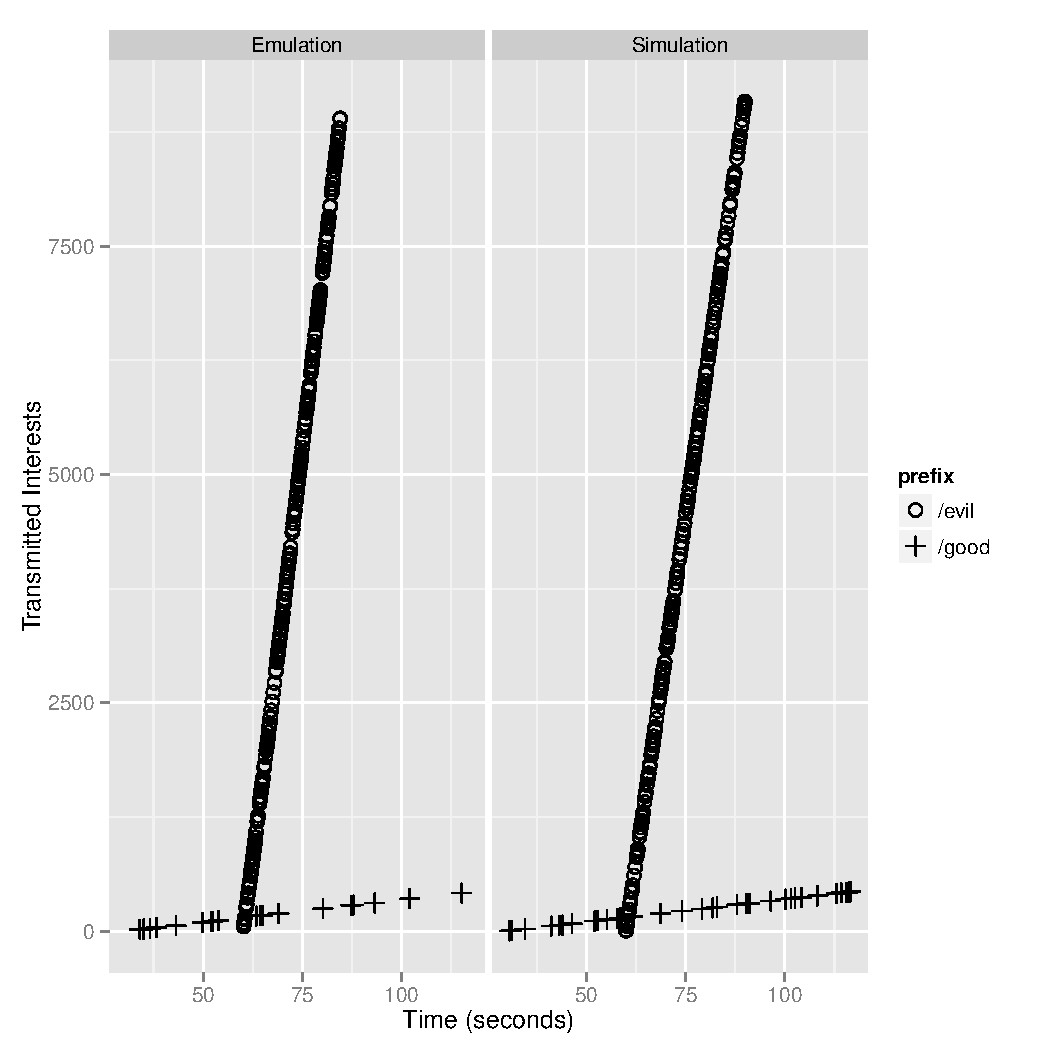
\includegraphics[scale=0.5]{figures/sim-emu-power.pdf}
%  \caption{Strength of Interest flooding attack}
%  \label{fig:simemupower}
%\end{figure}

%\begin{figure}[htpb]
%  \centering
%  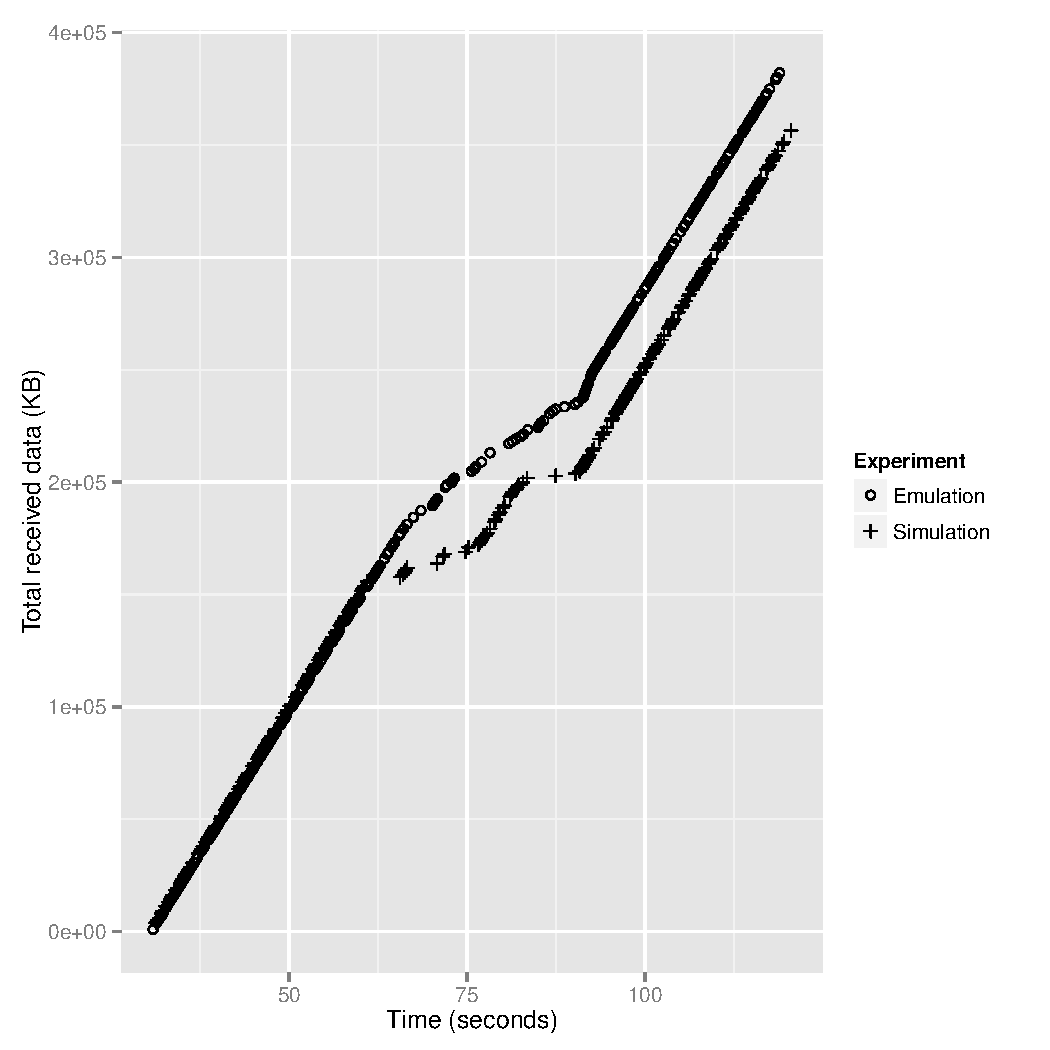
\includegraphics[scale=0.5]{figures/sim-emu-performance.pdf}
%  \caption{Data retrieval by legitimate clients}
%  \label{fig:simemuperf}
%\end{figure}


%%% Local Variables: 
%%% mode: latex
%%% TeX-master: "paper"
%%% End: 
